\documentclass[12pt]{article}

\usepackage{graphicx}
\usepackage{paralist}
\usepackage{hyperref}
\usepackage{xspace}
\usepackage{amsfonts}
\usepackage{amsmath}
\usepackage{array}

\newcolumntype{P}[1]{>{\raggedright\arraybackslash}p{#1}}

\newcommand{\latex}{\LaTeX\xspace}

\oddsidemargin 0mm
\evensidemargin 0mm
\textwidth 160mm
\textheight 200mm
\renewcommand\baselinestretch{1.0}

\pagestyle {plain}
\pagenumbering{arabic}

\newcounter{stepnum}

\title{
    SFWRENG 2XB3 Final Project \\
    \large Design Specification\\
    \vspace{1ex}
    \large Department of Computing and Software\\
    \large McMaster University\\
    \vspace{1ex}
    \large Group 8\\
    \large Project Name: NavSafe\\
    \large Version Number: 1.0
}

\author{
    Arkin Modi - 400142497\\
    Benson Hall - 400129627\\
    Joy Xiao - 400125285\\
    Leon So - 400127468\\
    Timothy Choy - 400135272
}
\date{Last updated: April 12, 2019}

\begin{document}
\maketitle
\newpage

\section{Revision}
    \subsection{Team Members and Responsibilities}
    \begin{tabular}{|l|l|l|}
    \hline
    \textbf{Team Member} & \textbf{Student Number} & \textbf{Responsibilities}\\
    \hline
    Arkin Modi & 400142497 & Head of Back-End\\
    \hline
    Benson Hall & 400129627 & Team Leader, Scrum Leader, Back-End Programmer\\
    \hline
    Leon So & 400127468 & Back-End Programmer\\
    \hline
    Timothy Choy & 400135272 & Head of Front-End and Programmer\\
    \hline
    Joy Xiao & 400125285 & Log Admin and Back-End Programmer\\
    \hline
    \end{tabular}

    \subsection{Revision History}
    \begin{tabular}{|l|l|}
        \hline
        \textbf{Date} & \textbf{Changes}\\
        \hline
        March 7, 2019 & Added skeleton\\
        \hline
        April 12, 2019 & Added content to all sections\\
        \hline
    \end{tabular}

    \subsection{Attestation and Consent}
    \textit{By virtue of submitting this document we electronically sign and date that the work being submitted by all the individuals in the group is their exclusive work as a group and we consent to make available the application developed through [CS] or [SE]-2XB3 project, the reports, presentations, and assignments (not including my name and student number) for future teaching purposes.}
\newpage

\section{Contribution}
\begin{tabular}{|P{2.5cm}|P{4cm}|P{5cm}|P{3.5cm}|}
    \hline
    \textbf{Name} & \textbf{Role(s)} & \textbf{Contributions} & \textbf{Comments}\\
    \hline
    Arkin Modi & Head of Back-End & Requirements Specification, Design Specification & ~\\
    \hline
    Benson Hall & Team Leader, Scrum Leader, Back-End Programmer & Graph construction and associated "shortest-path" algorithm, project log. %Design Specification - this is mildly subjective as of now
    & ~\\
    \hline
    Leon So & Back-End Programmer & All read modules, Collision ADT, Intersection ADT, Street ADT, both searching algorithm (SearchIntersections.java, SearchCollisions.java), Top-down MergeSort for sorting intersections alphabetically, Top-down MergeSort for sorting collisions by severity codes, fatalities, and injuries. & ~\\
    \hline
    Timothy Choy & Head of Front-End and Programmer & Project Log, Everything to do with front end (designing the interface, Google Maps API integration, connecting front end to back end), Decomposition Tree & ~\\
    \hline
    Joy Xiao & Log Admin and Back-End Programmer & Project Log, Top-Down MergeSort for sorting the collisions according to their severity, fatalities, number of severe injuries, then number of injuries, created the unit testing for all the read modules, searching modules, and sorting modules. &~\\
    \hline
\end{tabular}
\newpage

\section{Executive Summary}
The purpose of NavSafe is to provide a path from a start point to an end point in the City of Seattle. This path however will be generated with past collisions data to improve the safety of the path. Traveling in a city can be dangerous, and accidents tend to happen particular stops in the city. Vehicle collisions can lead to injuries or even death. Mistakes by pedestrian or driver can lead to a higher chance of a fatal collision in these intersections. With this trend we can use past data to plot a path avoiding this areas. This is done by assigning a safety weighting to each street and intersection. Using this, we can calculate the shortest safest path.

\newpage

\tableofcontents
\newpage

\section{Design Overview}
    \subsection{Decomposition Explanation}
    %Explanation of why you have decomposed the application into those classes.
    NavSafe is broken down into four major sections, Data Types, Read, Graph and Search/Sort. The Data Types are used to organize the data into a form that is more usable to the developer. This section contains the Collision, Intersections and Street modules.\\
    
    \noindent The Read section is broken down into four modules. The ReadWrite module is more of a pre-processor with removes usable data in our data sets. The other three modules, ReadCollisions, ReadIntersections and ReadStreets are used to read and parse the data from the data sets.\\
    
    \noindent The Graph section is broken down into five modules, EdgeWeightedGraph, IndexMinPQ, MakeGraph, WeightedEdge and DijkstraSP. These are used to find the shortest safest path from point A to point B.\\
    
    \noindent The Search/Sort section is broken down into three modules, SearchCollision, SearchIntersections and SortIntersectionDropDown. These are primarly used for their own independent features in the front-end.\\
    
    \noindent The reasoning to why the program was decomposed into the four major sections is emphasis the idea of separation of concerns. We also wanted to promote high cohesion and low coupling. With each module is closely related to the other modules in its respective section, we can achieve high cohesion. Also, by not having the modules be dependent on many other modules, which achieves low coupling. These are the reasons to why NavSafe was decomposed the was it was.
    
    \subsection{UML Class Diagram}
    %You should include a UML class diagram showing a static representation of your application classes and relationship between classes.
    \begin{center}
        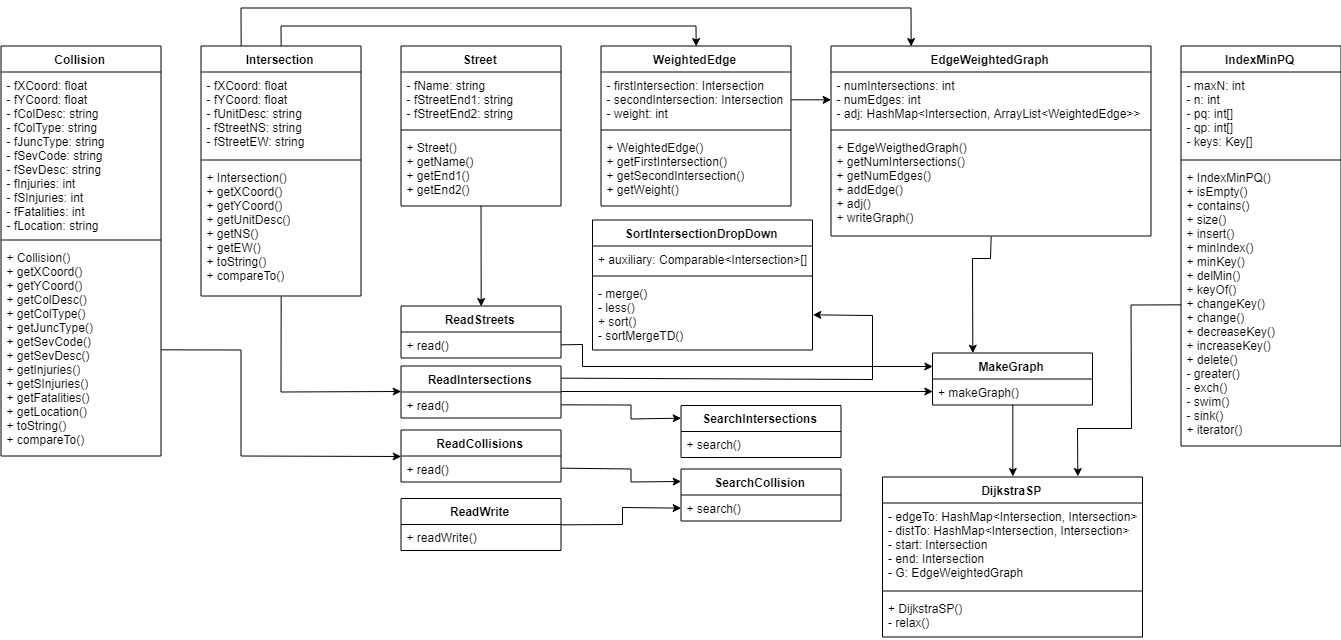
\includegraphics[angle=270, scale=0.4]{UML_Class_Diagram.png}
    \end{center}

\newpage
\section{Module Interface Specification}
\subsection{ReadWrite Module}
\subsection*{Module}
ReadWrite

\subsubsection*{Uses}
None

\subsubsection*{Trace Back to Requirements}
This is a part of the Read Module. This helps with Accuracy of Results by removing inaccurate data.

\subsection*{Syntax}
\subsubsection*{Exported Access Programs}
    \begin{tabular}{|l|l|l|l|}
    \hline
    \textbf{Routine Name} & \textbf{In} & \textbf{Out} & \textbf{Exceptions}\\
    \hline
    readWrite & ~ & ~ & ~\\
    \hline
    \end{tabular}
    
\subsection*{Semantics}
\subsubsection*{Environment Variables}
collisionData: File containing the data set of collisions

\subsubsection*{State Variables}
None

\subsubsection*{Assumptions}
The collisionData file will not change format.

\subsubsection*{Access Routine Semantics}

readWrite():
\begin{itemize}
    \item transition: All the rows missing any data are removed from collisionData
\end{itemize}

\newpage
\subsection{Read Intersections Module}
\subsection*{Module}
ReadIntersections

\subsubsection*{Uses}
Intersection

\subsubsection*{Trace Back to Requirements}
This is a part of the Read Module. This helps with Accuracy of Results by taking only the data we need.

\subsection*{Syntax}
\subsubsection*{Exported Access Programs}
    \begin{tabular}{|l|l|l|l|}
    \hline
    \textbf{Routine Name} & \textbf{In} & \textbf{Out} & \textbf{Exceptions}\\
    \hline
    read & ~ & seq of Intersections & ~\\
    \hline
    \end{tabular}
    
\subsection*{Semantics}
\subsubsection*{Environment Variables}
intersectionData: File containing the data set of intersections

\subsubsection*{State Variables}
None

\subsubsection*{Assumptions}
The intersectionData file will not change format.

\subsubsection*{Access Routine Semantics}

read():
\begin{itemize}
    \item output: A sequence of intersections where each intersection is parsed from each line in the IntersectionData file
\end{itemize}

%insert UMLSM-ReadIntersections.png here
\subsubsection*{UML State Machine}
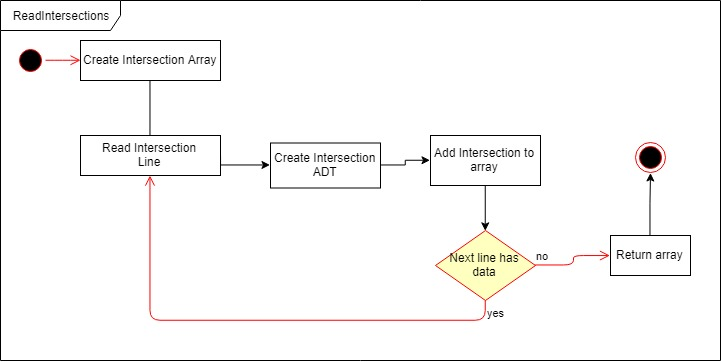
\includegraphics[scale=0.625]{UMLSM-ReadIntersections.png}

\newpage
\subsection{Read Streets Module}
\subsection*{Module}
ReadStreets

\subsubsection*{Uses}
Streets

\subsubsection*{Trace Back to Requirements}
This is a part of the Read Module. This helps with Accuracy of Results by taking only the data we need.

\subsection*{Syntax}
\subsubsection*{Exported Access Programs}
    \begin{tabular}{|l|l|l|l|}
    \hline
    \textbf{Routine Name} & \textbf{In} & \textbf{Out} & \textbf{Exceptions}\\
    \hline
    read & ~ & seq of Streets & ~\\
    \hline
    \end{tabular}
    
\subsection*{Semantics}
\subsubsection*{Environment Variables}
streetData: File containing the data set of streets

\subsubsection*{State Variables}
None

\subsubsection*{Assumptions}
The streetData file will not change format.

\subsubsection*{Access Routine Semantics}

read():
\begin{itemize}
    \item output: A sequence of streets where each street is parsed from each line in the streetData file
\end{itemize}

\newpage
\subsection{Read Collisions Module}
\subsection*{Module}
Read

\subsubsection*{Uses}
Collision

\subsubsection*{Trace Back to Requirements}
This is a part of the Read Module. This helps with Accuracy of Results by taking only the data we need.

\subsection*{Syntax}
\subsubsection*{Exported Access Programs}
    \begin{tabular}{|l|l|l|l|}
    \hline
    \textbf{Routine Name} & \textbf{In} & \textbf{Out} & \textbf{Exceptions}\\
    \hline
    read & ~ & seq of Collisions & ~\\
    \hline
    \end{tabular}
    
\subsection*{Semantics}
\subsubsection*{Environment Variables}
collisionData: File containing the data set of collisions

\subsubsection*{State Variables}
None

\subsubsection*{Assumptions}
The collisionData file will not change format.

\subsubsection*{Access Routine Semantics}

read():
\begin{itemize}
    \item output: A sequence of collisions where each collision is parsed from each line in the collisionData file
\end{itemize}

\newpage
\subsection{Intersection Module}
\subsection*{Module}
Intersection

\subsubsection*{Uses}
None

\subsubsection*{Trace Back to Requirements}
This helps with Reliability as it makes it easier for the developer to get the required data. This will also improve Maintability.

\subsection*{Syntax}
\subsubsection*{Exported Types}
None

\subsubsection*{Exported Constants}
None

\subsubsection*{Exported Access Programs}
    \begin{tabular}{|l|l|l|l|}
    \hline
    \textbf{Routine Name} & \textbf{In} & \textbf{Out} & \textbf{Exceptions}\\
    \hline
    new Intersection & seq of string & Intersection & ~\\
    \hline
    getXCoord & ~ & float & ~\\
    \hline
    getYCoord & ~ & float & ~\\
    \hline
    getUnitDesc & ~ & string & ~\\
    \hline
    getNS & ~ & string & ~\\
    \hline
    getEW & ~ & string & ~\\
    \hline
    toString & ~ & string & ~\\
    \hline
    compareTo & Intersection & int & ~\\
    \hline
    \end{tabular}
    
\subsection*{Semantics}
\subsubsection*{State Variables}
fXCoord: X-coordinate of intersection location\\
fYCoord: Y-coordinate of intersection location\\
fUnitDesc: Intersection description\\
fStreetNS: Street in north-south direction\\
fStreetEW: Street in east-west direction

\subsubsection*{Access Routine Semantics}

\noindent Intersection(s):
\begin{itemize}
    \item transition: fXCoord, fYCoord, fUnitDesc, fStreetNS, fStreetEW := float(s[0]), float(s[1]), s[2], s[3], s[4]
\end{itemize}

\noindent getXCoord():
\begin{itemize}
    \item output: out := fXCoord
\end{itemize}

\noindent getYCoord():
\begin{itemize}
    \item output: out := fYCoord
\end{itemize}

\noindent getUnitDesc():
\begin{itemize}
    \item output: out := fUnitDesc
\end{itemize}

\noindent getNS():
\begin{itemize}
    \item output: out := fStreetNS
\end{itemize}

\noindent getEW():
\begin{itemize}
    \item output: out := fStreetEW
\end{itemize}

\noindent toString():
\begin{itemize}
    \item output: out := "StreetNS: " + fStreetNS +" StreetEW: " + fStreetEW
\end{itemize}

\noindent compareTo(s):
\begin{itemize}
    \item output: out := compares intersection to s based on Unit Desc's letters (alphabetical order) and return -1 is less, 1 if greater, or 0 if equal
\end{itemize}

\newpage
\subsection{Collision Module}
\subsection*{Module}
Collision

\subsubsection*{Uses}
None

\subsubsection*{Trace Back to Requirements}
This helps with Reliability as it makes it easier for the developer to get the required data. This will also improve Maintability.

\subsection*{Syntax}
\subsubsection*{Exported Types}
None

\subsubsection*{Exported Constants}
None

\subsubsection*{Exported Access Programs}
    \begin{tabular}{|l|l|l|l|}
    \hline
    \textbf{Routine Name} & \textbf{In} & \textbf{Out} & \textbf{Exceptions}\\
    \hline
    new Collision & seq of string & Collision & ~\\
    \hline
    getXCoord & ~ & float & ~\\
    \hline
    getYCoord & ~ & float & ~\\
    \hline
    getColDesc & ~ & string & ~\\
    \hline
    getColType & ~ & string & ~\\
    \hline
    getJuncType & ~ & string & ~\\
    \hline
    getSevCode & ~ & string & ~\\
    \hline
    getSevDesc & ~ & string & ~\\
    \hline
    getInjuries & ~ & int & ~\\
    \hline
    getSInjuries & ~ & int & ~\\
    \hline
    getFatalities & ~ & int & ~\\
    \hline
    getLocation & ~ & string & ~\\
    \hline
    toString & ~ & string & ~\\
    \hline
    compareTo & Collision & int & ~\\
    \hline
    \end{tabular}
    
\subsection*{Semantics}
\subsubsection*{State Variables}
fXCoord: X-coordinate of collision location\\
fYCoord: Y-coordinate of a collision location\\
fColDesc: Collision description\\
fColType: Collision type\\
fJuncType: Junction type\\
fSevCode: Severity code\\
fSevDesc: Severity description\\
fInjuries: number of injuries\\
fSInjuries: number of serious injuries\\
fFatalities: number of fatalities\\
fLocation: Location of collision

\subsubsection*{Access Routine Semantics}

\noindent Collision(s):
\begin{itemize}
    \item transition: fXCoord, fYCoord, fColDesc, fColType, fJuncType, fSevCode, fSevDesc, fInjuries, fSInjuries, fFatalities, fLocation := float(s[0]), float(s[1]), s[2], s[3], s[4], s[5], s[6], int(s[7]), int(s[8]), int(s[9]), s[10]
\end{itemize}

\noindent getXCoord():
\begin{itemize}
    \item output: out := fXCoord
\end{itemize}

\noindent getYCoord():
\begin{itemize}
    \item output: out := fYCoord
\end{itemize}

\noindent getColDesc():
\begin{itemize}
    \item output: out := fColDesc
\end{itemize}

\noindent getColType():
\begin{itemize}
    \item output: out := fColType
\end{itemize}

\noindent getJuncType():
\begin{itemize}
    \item output: out := fJuncType
\end{itemize}

\noindent getSevCode():
\begin{itemize}
    \item output: out := fSevCode
\end{itemize}

\noindent getSevDesc():
\begin{itemize}
    \item output: out := fSevDesc
\end{itemize}

\noindent getInjuries():
\begin{itemize}
    \item output: out := fInjuries
\end{itemize}

\noindent getSInjuries():
\begin{itemize}
    \item output: out := fSInjuries
\end{itemize}

\noindent getFatalities():
\begin{itemize}
    \item output: out := fFatalities
\end{itemize}

\noindent getLocation():
\begin{itemize}
    \item output: out := fLocation
\end{itemize}

\noindent toString():
\begin{itemize}
    \item output: out := "X-coord: " + fXCoord + " Y-coord: " + fYCoord + " Collision Description: " + fColDesc + " Collision Type: " + fColType + " Junction Type: " + fJuncType + " Light Condition: " + " Severe Injuries: " + fSInjuries + " Severity Code: " + fSevCode + " Fatalities: " + fFatalities + " Injuries: " + fInjuries
\end{itemize}

\noindent compareTo(s):
\begin{itemize}
    \item output: out := Compares collision to s based on number of severity code, then fatalities, then serious injuries, then number of injuries and return -1 is less, 1 if greater, or 0 if equal
\end{itemize}

\newpage
\subsection{Street Module}
\subsection*{Module}
Street

\subsubsection*{Uses}
None

\subsubsection*{Trace Back to Requirements}
This helps with Reliability as it makes it easier for the developer to get the required data. This will also improve Maintability.

\subsection*{Syntax}
\subsubsection*{Exported Types}
None

\subsubsection*{Exported Constants}
None

\subsubsection*{Exported Access Programs}
    \begin{tabular}{|l|l|l|l|}
    \hline
    \textbf{Routine Name} & \textbf{In} & \textbf{Out} & \textbf{Exceptions}\\
    \hline
    new Street & seq of string & Street & ~\\
    \hline
    getName & ~ & string & ~\\
    \hline
    getEnd1 & ~ & string & ~\\
    \hline
    getEnd2 & ~ & string & ~\\
    \hline
    \end{tabular}
    
\subsection*{Semantics}
\subsubsection*{State Variables}
fName: Street Name\\
fStreetEnd1: One end of the street\\
fStreetEnd2: One end of the street

\newpage
\subsubsection*{Access Routine Semantics}
\noindent Street(s):
\begin{itemize}
    \item transition: fName, fStreetEnd1, fStreetEnd2 := s[0], s[1], s[2]
\end{itemize}

\noindent getName():
\begin{itemize}
    \item output: out := fName
\end{itemize}

\noindent getEnd1():
\begin{itemize}
    \item output: out := fStreetEnd1
\end{itemize}

\noindent getEnd2():
\begin{itemize}
    \item output: out := fStreetEnd2
\end{itemize}

\newpage
\subsection{Search Intersection Module}
\subsection*{Module}
SearchIntersections

\subsubsection*{Uses}
Intersection\\
ReadIntersections

\subsubsection*{Trace Back to Requirements}
This is part of the Search Module. This helps with Accuracy of Results as this module will guranntee the result is accurate.

\subsection*{Syntax}
\subsubsection*{Exported Types}
None

\subsubsection*{Exported Constants}
None

\subsubsection*{Exported Access Programs}
    \begin{tabular}{|l|l|l|l|}
    \hline
    \textbf{Routine Name} & \textbf{In} & \textbf{Out} & \textbf{Exceptions}\\
    \hline
    search & string, string, string & seq of Integer & ~\\
    \hline
    \end{tabular}
    
\subsection*{Semantics}
\subsubsection*{State Variables}
None

\subsubsection*{Access Routine Semantics}
\noindent search(x, y, z):
\begin{itemize}
    \item output: returns the index of two Intersections where the first index contains x and y, and the second index contains x and z
\end{itemize}

\newpage
\subsection{Search Collision Module}
\subsection*{Module}
SearchCollision

\subsubsection*{Uses}
ReadWrite\\
Collision\\
Read

\subsubsection*{Trace Back to Requirements}
This is part of the Search Module. This helps with Accuracy of Results as this module will guarantee the result is accurate.

\subsection*{Syntax}
\subsubsection*{Exported Types}
None

\subsubsection*{Exported Constants}
None

\subsubsection*{Exported Access Programs}
    \begin{tabular}{|l|l|l|l|}
    \hline
    \textbf{Routine Name} & \textbf{In} & \textbf{Out} & \textbf{Exceptions}\\
    \hline
    search & Intersection, Intersection & Integer & ~\\
    \hline
    \end{tabular}
    
\subsection*{Semantics}
\subsubsection*{State Variables}
None

\newpage
\subsubsection*{Access Routine Semantics}
\noindent search(x, y):
\begin{itemize}
    \item output: searches for all collisions contained in street/edge between 2 intersections, x and y, and returns summed weight of all collisions calculated based on severity code
\end{itemize}

%insert UMLSM-SearchCollisions.png here.
\subsubsection*{UML State Machine}
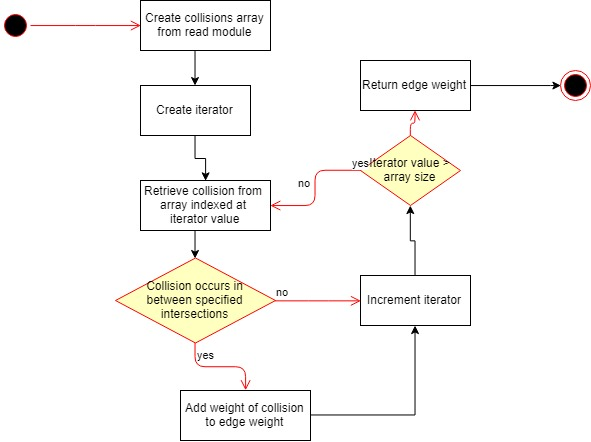
\includegraphics[scale=0.725]{UMLSM-SearchCollision.png}

\newpage
\subsection{Sort Intersection Module}
\subsection*{Module}
SortIntersectionDropDown

\subsubsection*{Uses}
ReadInsertions

\subsubsection*{Trace Back to Requirements}
This is part of the Sort Module. This helps with Performance as this module utilizes an efficient algorithm. The faster run time also helps with Human-computer Interface Issues.

\subsection*{Syntax}
\subsubsection*{Exported Types}
None

\subsubsection*{Exported Constants}
None

\subsubsection*{Exported Access Programs}
    \begin{tabular}{|l|l|l|l|}
    \hline
    \textbf{Routine Name} & \textbf{In} & \textbf{Out} & \textbf{Exceptions}\\
    \hline
    sort & Comparable, Integer & ~ & ~\\
    \hline
    \end{tabular}
    
\subsection*{Semantics}
\subsubsection*{State Variables}
None

\subsubsection*{Access Routine Semantics}
\noindent sort(x, y):
\begin{itemize}
    \item transition: sorts the comparable in order of the predefined compareTo() method
\end{itemize}

\newpage
\subsection{Weighted Edge Module}
\subsection*{Module}
WeightedEdge

\subsubsection*{Uses}
Insertion

\subsubsection*{Trace Back to Requirements}
This is part of the Graph Module. This helps with Performance by creating a data structure that will reduce the search time for calculating the shortest path.

\subsection*{Syntax}
\subsubsection*{Exported Types}
None

\subsubsection*{Exported Constants}
None

\subsubsection*{Exported Access Programs}
    \begin{tabular}{|l|l|l|l|}
    \hline
    \textbf{Routine Name} & \textbf{In} & \textbf{Out} & \textbf{Exceptions}\\
    \hline
    new WeightedEdge & Intersection, Intersection, Integer & WeightedEdge & ~\\
    \hline
    getFirstIntersection & ~ & Intersection  & ~\\
    \hline
    getSecondIntersection & ~ & Intersection  & ~\\
    \hline
    getWeight & ~ & Integer  & ~\\
    \hline
    \end{tabular}
    
\subsection*{Semantics}
\subsubsection*{State Variables}
firstIntersection: The first intersection\\
secondIntersection: The second intersection\\
weight: The weight of the edge

\newpage
\subsubsection*{Access Routine Semantics}
\noindent WeightedEdge(x, y, z):
\begin{itemize}
    \item transition: firstIntersection, secondIntersection, weight := x. y. z
\end{itemize}

\noindent getFirstIntersection():
\begin{itemize}
    \item output: out := firstIntersection
\end{itemize}

\noindent getSecondIntersection():
\begin{itemize}
    \item output: out := secondIntersection
\end{itemize}

\noindent getWeight():
\begin{itemize}
    \item output: out := weight
\end{itemize}

\newpage
\subsection{Edge Weighted Graph Module}
\subsection*{Module}
EdgeWeightedGraph

\subsubsection*{Uses}
Insertion\\
WeightedEdge

\subsubsection*{Trace Back to Requirements}
This is part of the Graph Module. This helps with Performance by creating a data structure that will reduce the search time for calculating the shortest path.

\subsection*{Syntax}
\subsubsection*{Exported Types}
None

\subsubsection*{Exported Constants}
None

\subsubsection*{Exported Access Programs}
    \begin{tabular}{|l|l|l|l|}
    \hline
    \textbf{Routine Name} & \textbf{In} & \textbf{Out} & \textbf{Exceptions}\\
    \hline
    new EdgeWeightedGraph &  Integer & EdgeWeightedGraph & IllegalArgumentException\\
    \hline
    getNumIntersections & ~ & Integer  & ~\\
    \hline
    getNumEdges & ~ & Integer  & ~\\
    \hline
    addEdge & ~ & ~  & ~\\
    \hline
    adj & Intersection & seq of WeightedEdge & ~\\
    \hline
    writeGraph & string & ~ & ~\\
    \hline
    \end{tabular}
    
\subsection*{Semantics}
\subsubsection*{Environment Variables}
output: A text file

\subsubsection*{State Variables}
numIntersections: Number of intersections\\
numEdges: Number of edges\\
adj: Hash Map of Intersection and seq of WeightedEdge

\subsubsection*{Access Routine Semantics}
\noindent EdgeWeightedGraph(n):
\begin{itemize}
    \item transition: numIntersections, numEdges := n, 0
    \item expection: n < 0 $\Rightarrow$ IllegalArgumentException
\end{itemize}

\noindent getNumIntersections():
\begin{itemize}
    \item output: out := numIntersections
\end{itemize}

\noindent getNumEdges():
\begin{itemize}
    \item output: out := numEdges
\end{itemize}

\noindent addEdge(x, y, z):
\begin{itemize}
    \item output: out := craete and add the weigthed edge between x and y to adj
\end{itemize}

\noindent adj(x):
\begin{itemize}
    \item output: out := adj[x]
\end{itemize}

\noindent writeGraph():
\begin{itemize}
    \item transistion: write the graph to output in a csv format
\end{itemize}

\newpage
\subsection{Make Graph Module}
\subsection*{Module}
MakeGraph

\subsubsection*{Uses}
EdgeWeightedGraph\\
ReadIntersections\\
ReadStreets

\subsubsection*{Trace Back to Requirements}
This is part of the Graph Module. This helps with Performance by creating a graph and saving it so that the other algorithms do not need to spend time building the graph.

\subsection*{Syntax}
\subsubsection*{Exported Types}
None

\subsubsection*{Exported Constants}
None

\subsubsection*{Exported Access Programs}
    \begin{tabular}{|l|l|l|l|}
    \hline
    \textbf{Routine Name} & \textbf{In} & \textbf{Out} & \textbf{Exceptions}\\
    \hline
    makeGraph &  ~ & ~ & ~\\
    \hline
    \end{tabular}
    
\subsection*{Semantics}
\subsubsection*{Environment Variables}
output: A text file

\subsubsection*{State Variables}
None

\subsubsection*{Access Routine Semantics}
\noindent makeGraph():
\begin{itemize}
    \item transition: create a EdgeWeightedGraph from ReadIntersections and ReadStreets and write the graph to output
\end{itemize}

\newpage
\subsection{Dijkstra Shortest Path Module}
\subsection*{Module}
DijkstraSP

\subsubsection*{Uses}
MakeGraph\\
IndexMinPQ

\subsubsection*{Trace Back to Requirements}
This is part of the Graph Module. This helps with Performance by utilizing an efficient algorithm. This reduces run time and improves Human-computer Interface Issues as well.

\subsection*{Syntax}
\subsubsection*{Exported Types}
None

\subsubsection*{Exported Constants}
None

\subsubsection*{Exported Access Programs}
    \begin{tabular}{|l|l|l|l|}
    \hline
    \textbf{Routine Name} & \textbf{In} & \textbf{Out} & \textbf{Exceptions}\\
    \hline
    new DijkstraSP & string, Intersection, Intersection & DijkstraSP & ~\\
    \hline
    \end{tabular}
    
\subsection*{Semantics}
\subsubsection*{State Variables}
edgeTo: Hash Map of edges\\
distTo: Hash Map of distances with the key being an Intersection and the value being the total weight of the path\\
G: EdgeWeightedGraph\\
start: start Intersection\\
end: end Intersection

\subsubsection*{Access Routine Semantics}
\noindent DijkstraSP(s, x, y):
\begin{itemize}
    \item transition: create the EdgeWeightedGraph G from the file s and relax(G, start)
\end{itemize}

\subsubsection*{Local Functions}

relax(G, start):
\begin{itemize}
    \item transition: if new shortest path found then update the adj for G and relax(G, node connected to start)
\end{itemize}

\newpage
\subsection{Minimum-Oriented Indexed Priority Queue Module}
Refer to: \url{https://algs4.cs.princeton.edu/code/edu/princeton/cs/algs4/IndexMinPQ.java.html}

\subsubsection*{Trace Back to Requirements}
This is part of the Graph Module. This helps with Performance by utilizing an efficient algorithm. This reduces run time and improves Human-computer Interface Issues as well.

\newpage
\section{Internal Design Review}
NavSafe was made with the principles learned in SFWRENG 2AA4 and the algorithm design ideas from SFWRENG 2C03. The decomposition of this program was done with the software engineering principles in mind. Having high cohesion and low coupling is good in terms of the design. By programming in a object-oriented style enabled us to utilize the separation of concerns principle. When it comes to the algorithm choices, we used the best algorithm available. The sorting is done with merge sort. The shortest path is done with Dijkstra's algorithm. When it came to search, because of our specific implementation, linear search was the only option available. This introduced a big increase to the running time of the program. The searching aspect to NavSafe is where we could improve the most.

\end{document}